%!TEX TS-program = pdflatex
%!TEX root = tesi.tex
%!TEX encoding = UTF-8 Unicode

%\begin{figure}[ht] % TODO remove me
%  \begin{center}
%    \begin{tabular}{ccc}
%
%  \begin{subfigure}{.3\linewidth}
%    \centering\includegraphics[width=\textwidth]{example-image}
%    \caption{}
%  \end{subfigure} &
%
%    \end{tabular}
%    \caption{Alcune carcasse Conformi}
%    \label{fig:esempi_conformi}
%  \end{center}
%\end{figure}



\chapter{Gli Autoencoder}

Breve intuizione sugli AE
\todo[inline]{TODO recap capitolo}

\section{La Struttura di un Autoencoder}
Un \textit{Autoencoder}(AE) è un particolare tipo di rete neurale.
Può essere diviso in due componenti: il primo viene chiamato \textit{encoder}, mentre il secondo prende il nome di \textit{decoder}.
Lo scopo dell'\textit{encoder} è codificare il dato in ingresso in una versione compressa.
Sia $n$ la dimensionalità dell'\textit{input}.
Quando il dato raggiunge il collo di bottiglia dell'AE, ovvero la parte centrale della rete, ha raggiunto il livello di massima compressione, sia $m$ la sua nuova dimensionalità con $m<n$.
Lo spazio $m$-dimensionale in cui l'informazione è stata mappata viene chiamato spazio latente o spazio nascosto.
Ora il dato può essere decompresso dal \textit{decoder}, in questo modo verrà riportato alle sue dimensioni originali, cioè mappato nello spazio $n$-dimensionale di partenza.

Visto dall'esterno, il compito di un \textit{autoencoder} è quello di ritornare un valore il più simile al dato in ingresso.
Durante l'allenamento, fissato $m$ con un valore che dipende dalla forma della rete, si vuole trovare il miglior spazio latente possibile.
Dove con migliore si intende quello spazio di cardinalità $m$ che permette di mantenere tutte le informazioni caratterizzanti dell'input.
Riformulando quanto detto: un'\textit{autoencoder} può essere visto come una funzione $f$ rassomigliante la funzione identità, ma al cui intero c'è un vincolo tale da rendere il compito di restituzione dell'\textit{input} non banale.

Come viene spiegato da Andrew Ng in \cite{ng_sparse_ae}, gli \textit{autoencoder} fanno parte degli algoritmi di apprendimento non supervisionato.
Cioè di quella classe di algoritmi, in contrapposizione a quelli ad apprendimento supervisionato, che non ha bisogno di dati etichettati; anzi vengono usati proprio per trovare nuovi pattern e correlazioni tra gli elementi del \textit{dataset}.
Come gli algoritmi \textit{K-Means} e \textit{DBSCAN}, entrambi di \textit{clustering}, permettono di raggruppare nuvole di punti con caratteristiche simili. % TODO citare?
%I gruppi così creati possono far risaltare degli andamenti dei dati 
Un AE è non supervisionato perché, a priori, non conosciamo la forma che verrà data allo spazio latente. % TODO espandere?

Gli \textit{autoencoder} più semplici sono composti da due \textit{layer fully connected}: il primo funge da \textit{encoder}, ha un numero di unità nascoste pari alla dimensione dello spazio latente; il secondo ha tante unità quanto la dimension e dell'\textit{input}, quindi funge da \textit{decoder}.
L'architettura appena descritta può essere osservata in figura~\ref{fig:semplice_ae}, notare la tipica forma a clessidra.

\begin{figure}[ht] % TODO rifare con tikz
  \begin{center}
    %\centering\includegraphics[width=.4\textwidth]{example-image}
    \centering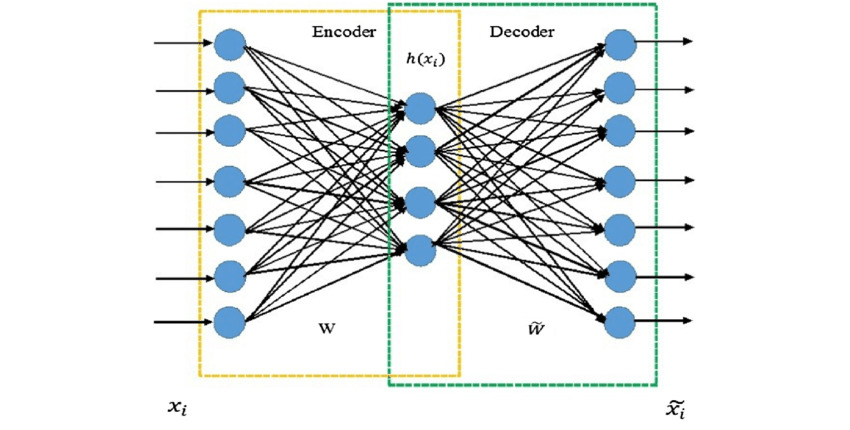
\includegraphics[width=\textwidth]{simple_ae}
  \end{center}
  \caption{Architettura di un semplice \textit{autoencoder}}
  \label{fig:semplice_ae}
\end{figure}

\todo[inline]{spiegare Conv, ConvTransposed, MaxPool, Upsampling}



\clearpage
\subsection{Applicazioni principali}

\paragraph{Denoising}

\paragraph{Variational}

\paragraph{Anomaly Detection}
